\subsection{AnimatedSprite}
A textured rectangle-shaped 1x1 Drawable that changes over time.

For different sizes use the scale in either the hum::Actor hum::Transform of
the Drawable's hum::Transform.

The AnimatedSprite plays the animation defined in the SpriteAnimation assigned to it.

For an example of usage of both AnimatedSprite and SpriteAnimation see the section 
of the SpriteAnimationManager\ref{lst:spriteAnimationManager}

\subsubsection{SpriteAnimation}

A SpriteAnimation models an animation built from a sequence of frames stored in a 
tilesheet.

Given the following tilesheet:
\begin{figure}[H]
    \centering
    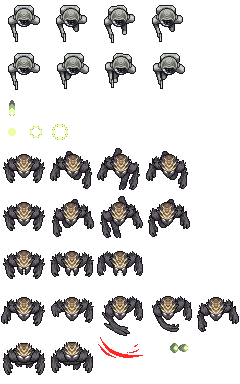
\includegraphics[width=0.7\textwidth]{sprites}
    \caption{sprites.png}
    \label{fig:sprites}
\end{figure}

The SpriteAnimation that stores the walking animation of the astronaut is defined 
in the next code fragment.

\begin{lstlisting}[caption=Astronaut walking animation]
mogl::SpriteAnimation walk{
  // texture containing the tilesheet
  game().getPlugin<mogl::MultimediaOGL>()->textures().get("sprites"),

  0,  // Horizontal offset of the tilesheet
  0,  // Vertical offset of the tilesheet
  0,  // Horizontal margin between tiles in the tilesheet
  0,  // Vertical margin between tiles in the tilesheet
  48, // Width of a tile in the tilesheet
  48, // Height of a tile in the tilesheet

  // Sequence of ids of the tiles in the tilesheet to play.
  {0, 1, 2, 3, 5, 6, 7, 8},

  // Sequence of hum::Times for each frame in the animation.
  std::vector(8, hum::Time::milliseconds(75))
};
\end{lstlisting}
